%%%%%%%%%%%%%%%%%%%%%%%%%%%%%%%%%%%%%%%%%%%%%%%%%%%%%%%%%%%%%%%%%%%%%%%%%%%%%%%
%                     Отчёт по лабораторной работе №4
%
% Дисциплина: Теория вероятностей и Математическая статистика
%                     
% Название:   Эмпирическая функция распределения и ядерные оценки
%
% Выполнил:   Михаил Маляренко
%
% Дата:       28 Ноя. 2020
%
%%%%%%%%%%%%%%%%%%%%%%%%%%%%%%%%%%%%%%%%%%%%%%%%%%%%%%%%%%%%%%%%%%%%%%%%%%%%%%%

% HEADER BEGIN 
\documentclass[12pt]{article}
\usepackage[utf8]{inputenc}
\usepackage[russian]{babel}
\usepackage{pscyr}
\usepackage[T2A]{fontenc}
\usepackage{geometry}
\usepackage{graphicx}
\usepackage{multirow}
\usepackage{amsmath}
\usepackage{amssymb}
\usepackage{hyperref}
\usepackage{xcolor}

\geometry {	
	a4paper, 
	left   = 20mm, 
	right  = 20mm, 
	top    = 20mm, 
	bottom = 20mm
}

\definecolor{urlcolor}{HTML}{2484BC} 
\definecolor{linkcolor}{HTML}{000000}

\graphicspath{{resource/}}
% HEADER END

% DIFINES BEGIN
\newcommand{\lskip}{\hfill\break}
% DEFINES END

\begin{document}

\begin{titlepage}
	\begin{center}
		\hfill \break
		{\textbf{Санкт-Петербургский политехнический университет Петра Великого}}\\
		\hfill \break
		\textbf{Институт прикладной математики и механики}\\
		 \hfill \break
		\textbf{Кафедра <<Телематика (при ЦНИИ РТК)>>}\\
		\vfill
		\large{\bfseries Отчет по лабораторной работе}\\
		\hfill \break
		\hfill \break
		\hfill \break
		\hfill \break
		\normalsize{\bfseries Эмпирические функции распределения и ядерные оценки}\\
		По дисциплине <<Теория вероятностей и Математическая статистика>>\\
		\hfill \break
		\hfill \break
		\hfill \break
	\end{center}
 
	\normalsize
	{ 
		\begin{tabular}{lp{2cm}cr}
			Выполнил &&&\\
			Студент гр. 3630201/80101&&\underline{\hspace{1.5cm}}& М.Д. Маляренко\\\\
			Руководитель&&&\\ 
			к.ф.-м.н., доцент && \underline{\hspace{1.5cm}}& А.Н. Баженов \\\\
			&&&<<\underline{\phantom{333}}>>\underline{\phantom{сентября000}}
			2020г.
		\end{tabular}
	}
\vfill

\begin{center} Санкт-Петербург \\2020 \end{center}
\end{titlepage}

\newpage

\setcounter{page}{2}

\begin{flushleft}

\setlength{\parindent}{1cm}

% TABLE OF CONTENTS
\tableofcontents

\newpage

% LIST OF FIGURES
\listoffigures

\newpage

\section{Постановка задачи}
    
	Заданы 5 распределений случайных величин:

	\begin{enumerate}
		\item Нормальное распределение $N(x, 0, 1)$
		\item Распределение Коши $C(x, 0, 1)$
		\item Распределение Лапласа $L(x, 0, 1/\sqrt{2})$
		\item Дискретное распределение Пуассона $P(k, 10)$
		\item Равномерное распределение $U(x, -\sqrt{3}, \sqrt{3})$
	\end{enumerate}

    \noindentДля каждого распределения необходимо сгенерировать выборки размером в 20, 60 и 100 элементов. На этих выборках построить эмпирические функции распределения. Также для выборок построить ядерные оценки на нормальном (гауссовом) ядре с тремя параметрами сглаживания: $h_n / 2$, $h_n$ и $2h_n$, где $h_n$ -- полоса пропускания, рассчитанная по эмпирическому правилу Сильвермана.
    
    Все графики необходимо строить на промежутке $[-4, 4]$ для непрерывных распределений и на $[6, 14]$ для дискретного распределения Пуассона.

\newpage

\section{Теория}

    \subsection{Эмпирическая функция распределения}

        Эмпирической (выборочной) функцией распределения называется относительная частота события $X < x$, полученная по данной выборке:\cite{theory1}

        $$
            F^*_n(x) = P^*(X < x)
            \label{ecdf1}
        $$

        Для расчета эмпирической функции распределения необходимо составить по выборке статистический ряд и просуммировать все частоты $n_i$, для которых элементы $x_i < x$:

        \begin{equation}
            F^*_n(x) = \frac{1}{n} \sum_{x_i < x} n_i
            \label{ecdf2}
        \end{equation}

    \subsection{Ядерные оценки}

        Оценка плотности вероятности $f(x)$ -- функция $\hat{f}_n(x)$, построенная на основе выборки $x_1, \dots, x_n$, представимая суммой:
        
        \begin{equation}
            \hat{f}_n(x) = \frac{1}{nh_n} \sum_{i = 1}^nK(\frac{x - x_i}{h_n})
            \label{kernel_est}
        \end{equation}

        В формуле (\ref{kernel_est}) $K(u)$ -- ядерная функция, $\{h_n\}$ -- последовательность положительных чисел, для которой

        $$
            h_n \xrightarrow[n \to \infty]{} 0 \qquad \frac{h_n}{n^{-1}} \xrightarrow[n \to \infty]{} \infty
        $$

       В данной лабораторной работе в качестве ядерной функции $K(u)$ используется гауссово ядро:

       \begin{equation}
           K(u) = \frac{1}{\sqrt{2\pi}}e^{-\frac{u^2}{2}}
           \label{guss_kernel}
       \end{equation}

       Для расчета полосы пропускания используется эмпирическое правило Сильвермана:\cite{theory2}

       \begin{equation}
           h_n = 1.06 \hat{\sigma}^{-1/5}
           \label{silverman}
       \end{equation}

       , где $\hat{\sigma}$ -- стандартное выборочное отклонение, $n$ -- размер выборки.

\newpage

\section{Реализация}

Расчёты и построение графиков производились в среде аналитических вычислений Maxima. Для построения ядерной оценки были написаны вспомогательные функции, параметрически задающие оценку плотности вероятности. Для построения графиков использовалась интегрированная в среду утилита gnuplot. Полный текст скрипта для среды Maxima представлен в репозитории GitHub.

\newpage

\section{Результаты}

    \subsection{Эмпирическая функция распределения}

       На рисунках 1-5 представлены графики, по которым можно визуально оценить отклонение эмпирической функции распределения (\ref{ecdf2}) с теоретической функций распределения.
       \lskip

        \begin{figure}[h]
        \begin{minipage}[h]{0.325\linewidth}
            \center{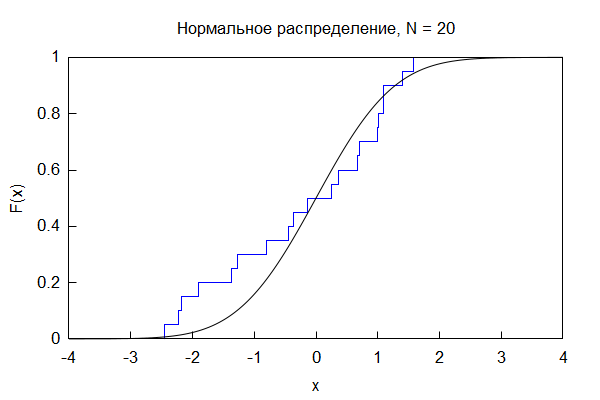
\includegraphics[width=1\linewidth]{N20.png}}
        \end{minipage}
        \begin{minipage}[h]{0.325\linewidth}
            \center{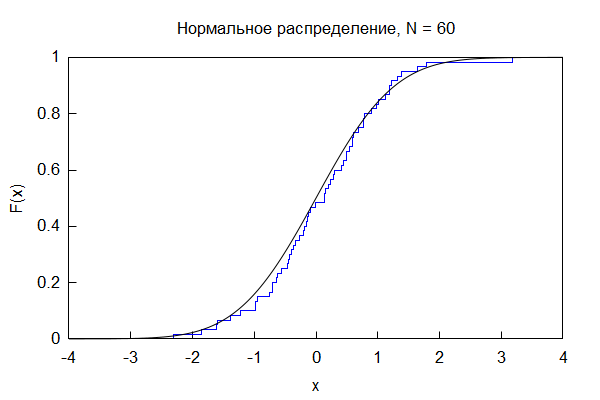
\includegraphics[width=1\linewidth]{N60.png}}
        \end{minipage}
        \begin{minipage}[h]{0.325\linewidth}
            \center{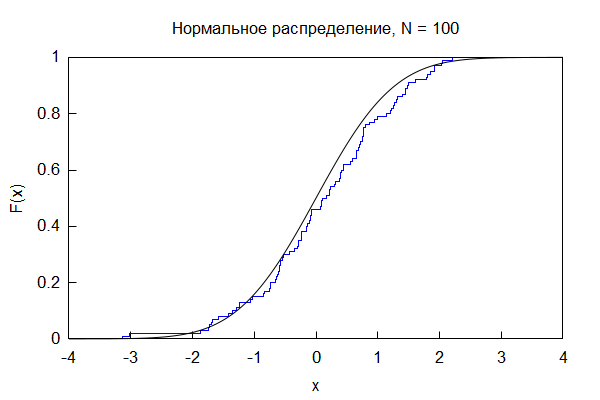
\includegraphics[width=1\linewidth]{N100.png}}
        \end{minipage}
        \caption{Эмпирическая функция нормального распределения $N(x, 0, 1)$}
        \end{figure}
        \lskip

        \begin{figure}[h]
        \begin{minipage}[h]{0.325\linewidth}
            \center{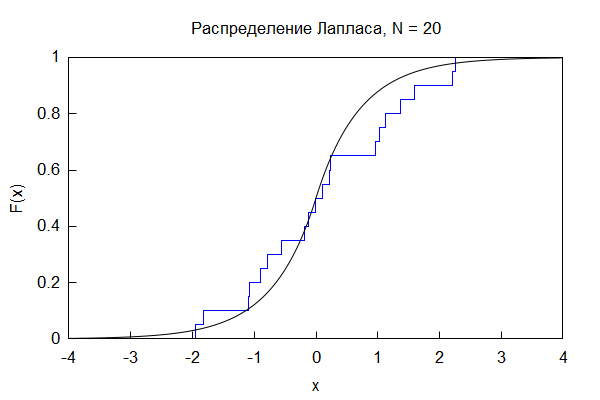
\includegraphics[width=1\linewidth]{L20.png}}
        \end{minipage}
        \begin{minipage}[h]{0.325\linewidth}
            \center{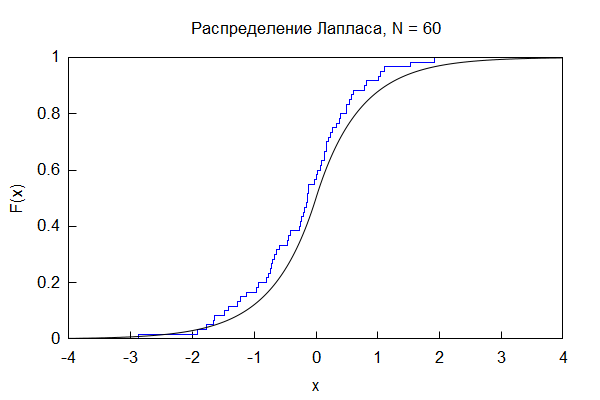
\includegraphics[width=1\linewidth]{L60.png}}
        \end{minipage}
        \begin{minipage}[h]{0.325\linewidth}
            \center{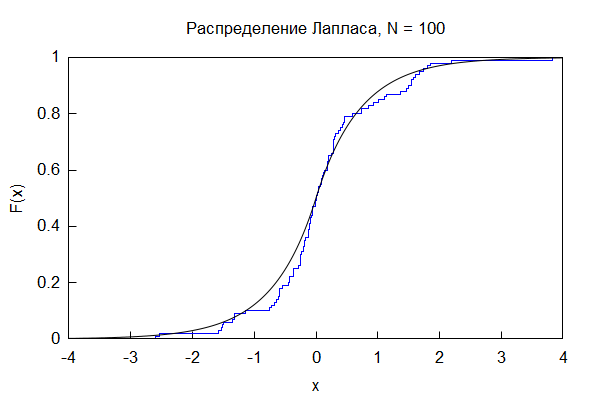
\includegraphics[width=1\linewidth]{L100.png}}
        \end{minipage}
        \caption{Эмпирическая функция распределения Лапласа $L(x, 0, 1/\sqrt{2})$}
        \end{figure}
        \lskip

        \begin{figure}[h]
        \begin{minipage}[h]{0.325\linewidth}
            \center{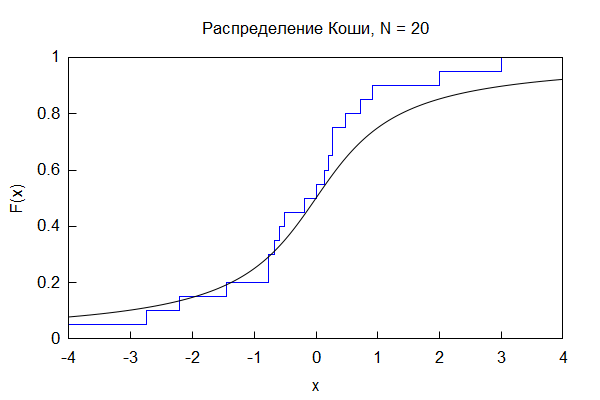
\includegraphics[width=1\linewidth]{C20.png}}
        \end{minipage}
        \begin{minipage}[h]{0.325\linewidth}
            \center{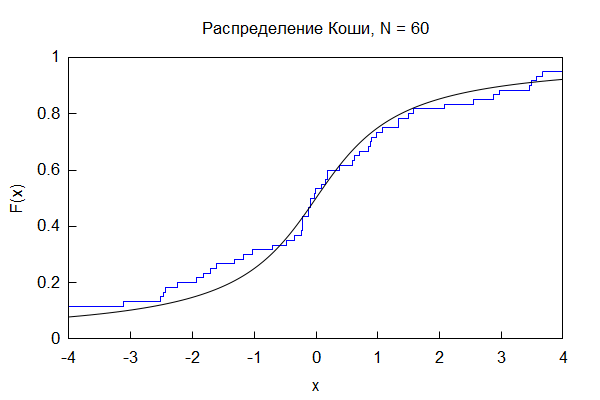
\includegraphics[width=1\linewidth]{C60.png}}
        \end{minipage}
        \begin{minipage}[h]{0.325\linewidth}
            \center{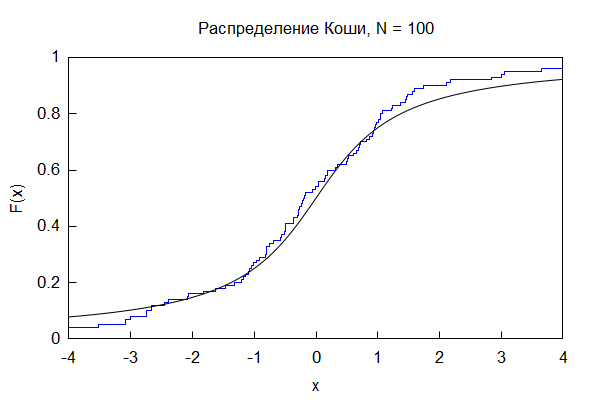
\includegraphics[width=1\linewidth]{C100.png}}
        \end{minipage}
        \caption{Эмпирическая функция распределения Коши $C(x, 0, 1)$}
        \end{figure}
        \lskip

        \newpage

        \begin{figure}[h]
        \begin{minipage}[h]{0.325\linewidth}
            \center{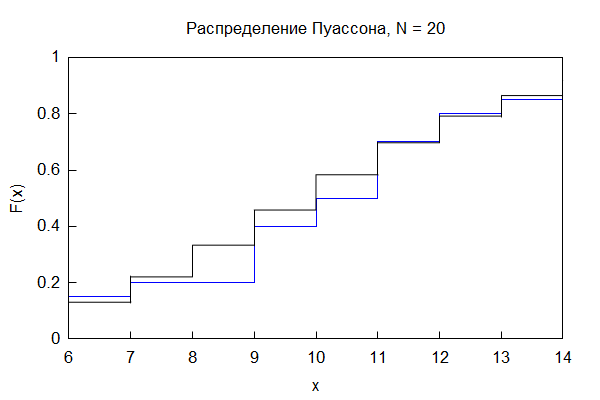
\includegraphics[width=1\linewidth]{P20.png}}
        \end{minipage}
        \begin{minipage}[h]{0.325\linewidth}
            \center{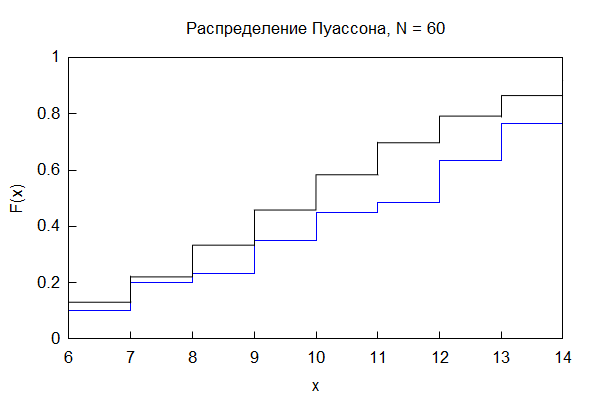
\includegraphics[width=1\linewidth]{P60.png}}
        \end{minipage}
        \begin{minipage}[h]{0.325\linewidth}
            \center{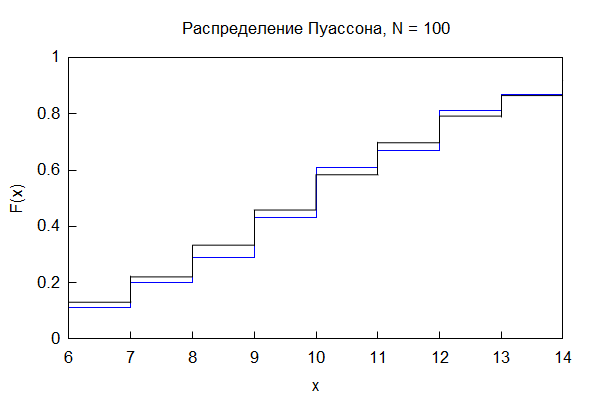
\includegraphics[width=1\linewidth]{P100.png}}
        \end{minipage}
        \caption{Эмпирическая функция распределения Пуассона $P(k, 10)$}
        \end{figure}
        \lskip

        \begin{figure}[h]
        \begin{minipage}[h]{0.325\linewidth}
            \center{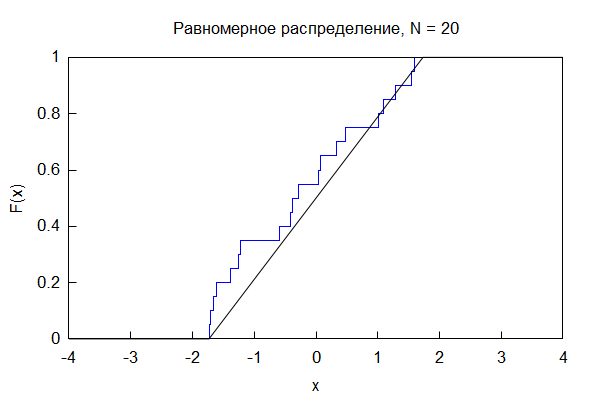
\includegraphics[width=1\linewidth]{U20.png}}
        \end{minipage}
        \begin{minipage}[h]{0.325\linewidth}
            \center{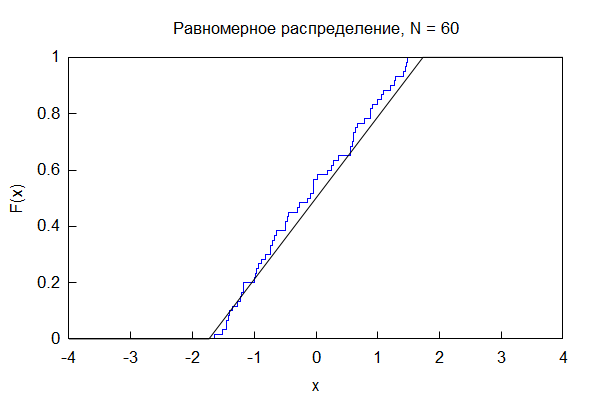
\includegraphics[width=1\linewidth]{U60.png}}
        \end{minipage}
        \begin{minipage}[h]{0.325\linewidth}
            \center{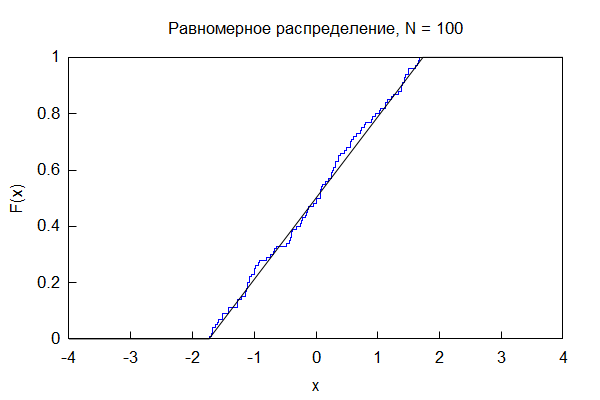
\includegraphics[width=1\linewidth]{U100.png}}
        \end{minipage}
        \caption{Эмпирическая функция равномерного распределения $U(x, -\sqrt{3}, \sqrt{3})$}
        \end{figure}

    \subsection{Ядерные оценки}

        На рисунках 6-10 представлены графики ядерных оценок плотности для выборок заданных распределений. Ядерная функция имеет вид (\ref{guss_kernel}). Черной пунктирной линией изображается теоретическая плотность вероятности, красной линии соответствует оценка с параметром сглаживания $h_n / 2$, зелёной -- с параметром $h_n$ и синей линии сответсвует оценка с параметром сглаживания $2h_n$. Параметр $h_n$ рассчитан согласно формуле (\ref{silverman}).
        \lskip
        \lskip

        \begin{figure}[h]
         \begin{minipage}[h]{0.325\linewidth}
             \center{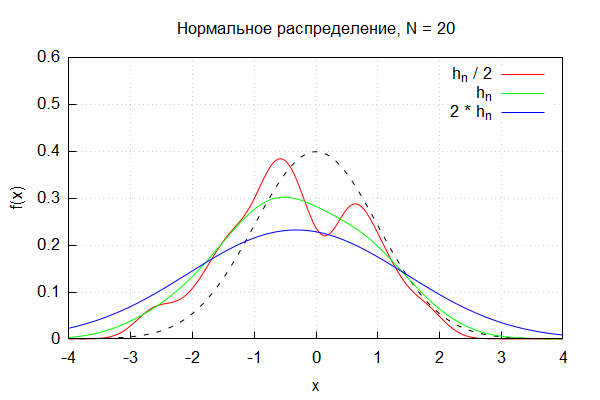
\includegraphics[width=1\linewidth]{fN20.png}}
         \end{minipage}
         \begin{minipage}[h]{0.325\linewidth}
             \center{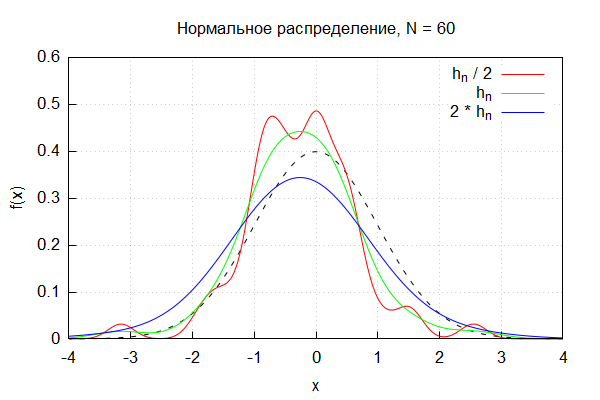
\includegraphics[width=1\linewidth]{fN60.png}}
         \end{minipage}
         \begin{minipage}[h]{0.325\linewidth}
             \center{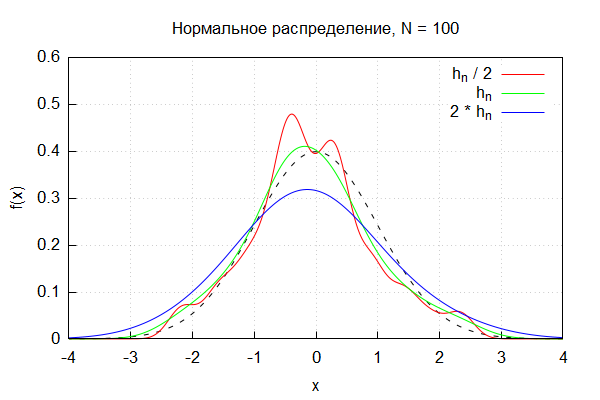
\includegraphics[width=1\linewidth]{fN100.png}}
         \end{minipage}
         \caption{Ядерная оценка плотности нормального распределения $N(x, 0, 1)$}
         \end{figure}
         \lskip

         \newpage
 
         \begin{figure}[h]
         \begin{minipage}[h]{0.325\linewidth}
             \center{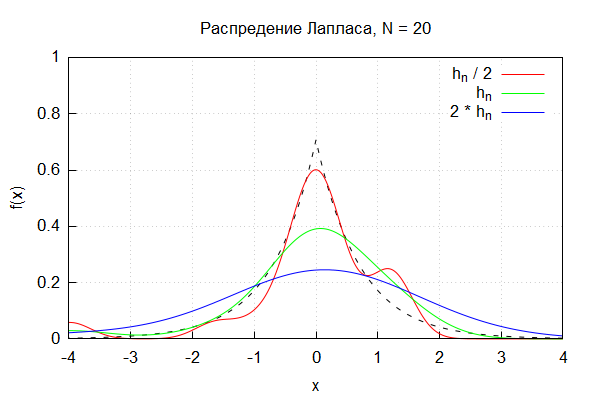
\includegraphics[width=1\linewidth]{fL20.png}}
         \end{minipage}
         \begin{minipage}[h]{0.325\linewidth}
             \center{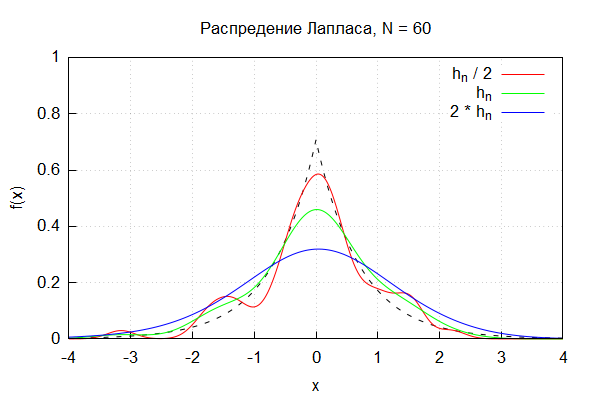
\includegraphics[width=1\linewidth]{fL60.png}}
         \end{minipage}
         \begin{minipage}[h]{0.325\linewidth}
             \center{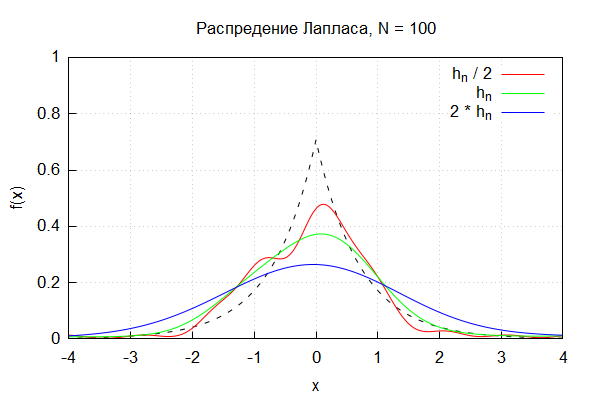
\includegraphics[width=1\linewidth]{fL100.png}}
         \end{minipage}
         \caption{Ядерная оценка плотности распределения Лапласа $L(x, 0, 1/\sqrt{2})$}
         \end{figure}
         \lskip
 
         \begin{figure}[h]
         \begin{minipage}[h]{0.325\linewidth}
             \center{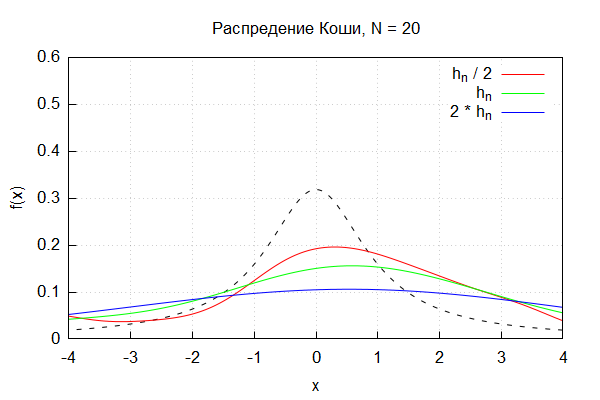
\includegraphics[width=1\linewidth]{fC20.png}}
         \end{minipage}
         \begin{minipage}[h]{0.325\linewidth}
             \center{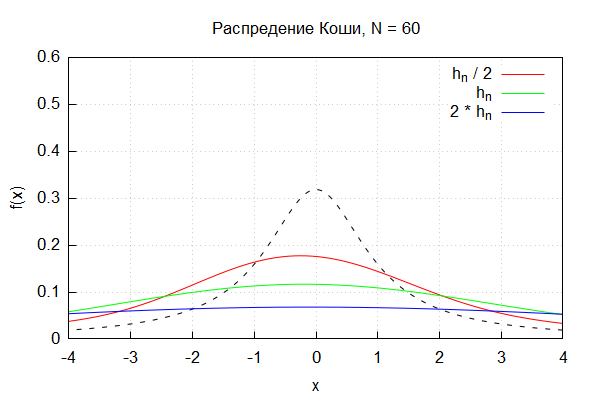
\includegraphics[width=1\linewidth]{fC60.png}}
         \end{minipage}
         \begin{minipage}[h]{0.325\linewidth}
             \center{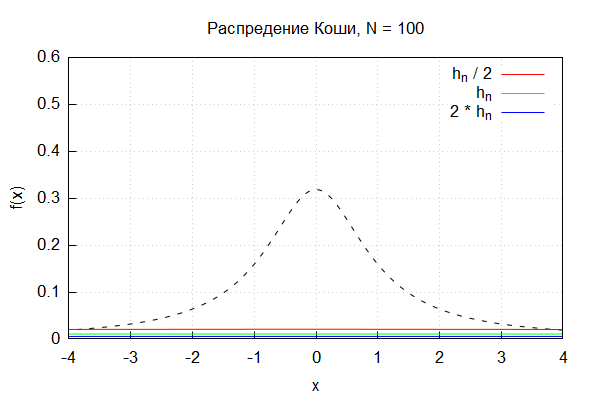
\includegraphics[width=1\linewidth]{fC100.png}}
         \end{minipage}
         \caption{Ядерная оценка плотности распределения Коши $C(x, 0, 1)$}
         \end{figure}
         \lskip
 
         \begin{figure}[h]
         \begin{minipage}[h]{0.325\linewidth}
             \center{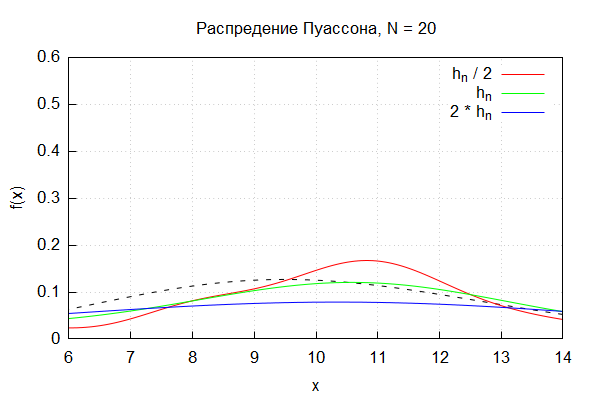
\includegraphics[width=1\linewidth]{fP20.png}}
         \end{minipage}
         \begin{minipage}[h]{0.325\linewidth}
             \center{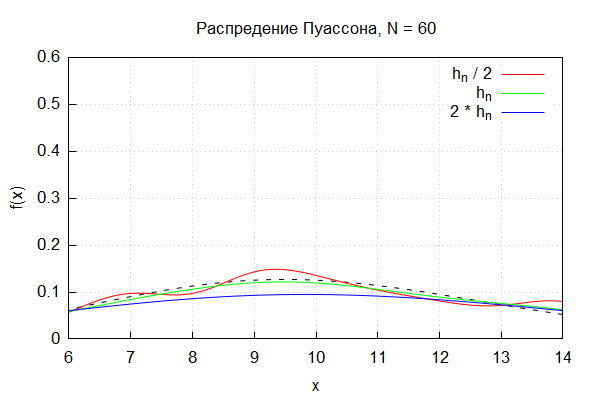
\includegraphics[width=1\linewidth]{fP60.png}}
         \end{minipage}
         \begin{minipage}[h]{0.325\linewidth}
             \center{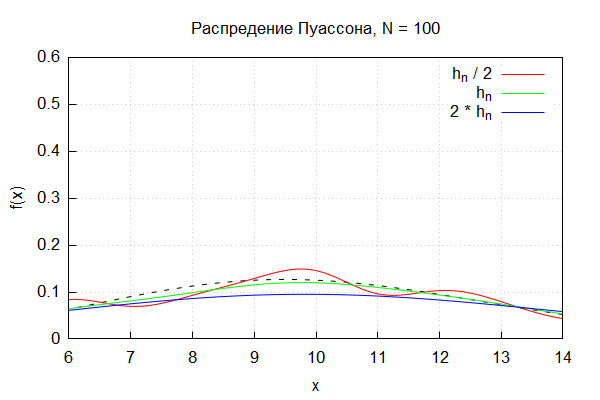
\includegraphics[width=1\linewidth]{fP100.png}}
         \end{minipage}
         \caption{Ядерная оценка плотности распределения Пуассона $P(k, 10)$}
         \end{figure}
         \lskip
 
         \begin{figure}[h!]
         \begin{minipage}[h]{0.325\linewidth}
             \center{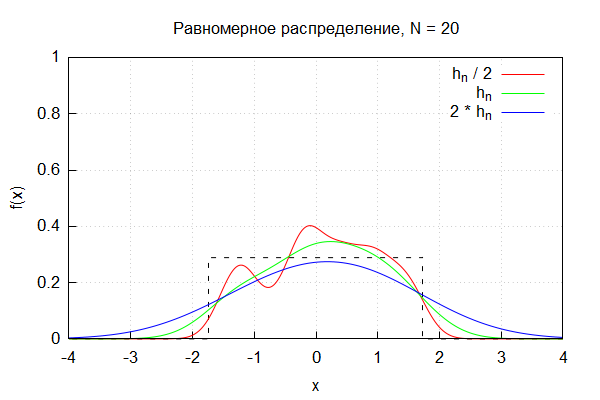
\includegraphics[width=1\linewidth]{fU20.png}}
         \end{minipage}
         \begin{minipage}[h]{0.325\linewidth}
             \center{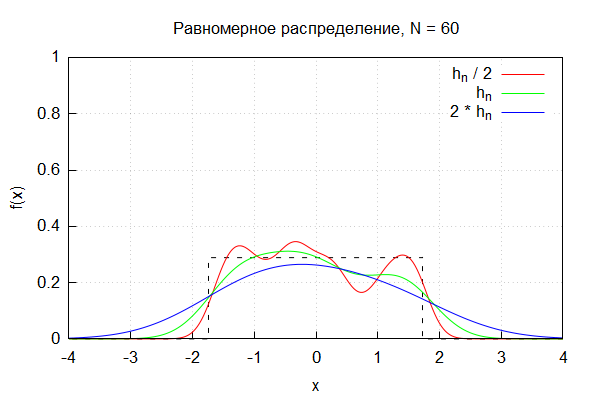
\includegraphics[width=1\linewidth]{fU60.png}}
         \end{minipage}
         \begin{minipage}[h]{0.325\linewidth}
             \center{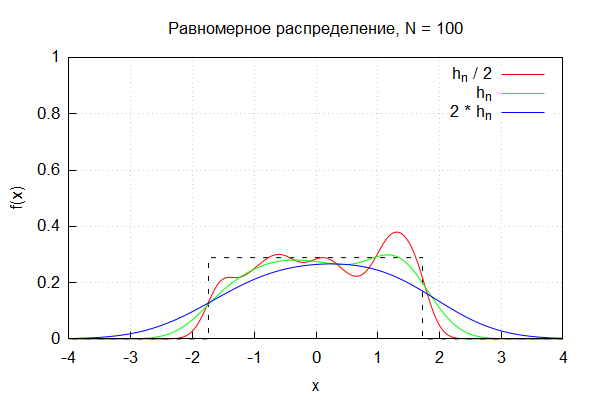
\includegraphics[width=1\linewidth]{fU100.png}}
         \end{minipage}
         \caption{Ядерная оценка плотности равномерного распределения $U(x, -\sqrt{3}, \sqrt{3})$}
         \end{figure}
         \lskip

\newpage

\section*{Заключение}
\addcontentsline{toc}{section}{Заключение}

        В результате выполнения лабораторной работы были построены эмпирические функции распределения для выборок, соответствующих заданным распределениям. По графикам видно, что чем больше мощность выборки, тем больше эмпириеская функция соответствует теоретической функции распределения.

        Также были построены ядерные оценки плотностей распределений. Относительно выбора полосы пропускания $h_n$ можно сделать вывод, что чем больше полоса пропускания, тем более сглажен график и менее чувствителен к отдельным частотам выборки. Для нормального распределения и распределении Пуассона наиболее подходит полоса пропускания $h_n$, полоса пропускания $h_n / 2$ точнее приближает ядерную оценку к теоретической плотности распределения Лапласа и равномерного распределения. Выборки, соответствующие распределению Коши, оценивать ядерными оценками не эффетивно ни при какой полосе пропускания.

\newpage

\addcontentsline{toc}{section}{Список литературы}

\begin{thebibliography}{9}

        \bibitem{theory1}
        Теоретическое приложение к лабораторным работам №1-4 по дисциплине «Математическая статистика». -- СПб.: СПбПУ, 2020. -- 12 c

        \bibitem{theory2} Амосова Н. Н., Куклин Б. А. и др. -- Вероятностные разделы математики. Учебник для бакалавров технических направлений. Под общей редакцией Ю. Д. Максимова -- СПб.: Иван Федоров, 2001. -- 589 с  
	
\end{thebibliography}

\newpage

\section*{Приложение А. Репозиторий с исходным кодом}
\addcontentsline{toc}{section}{Приложение А. Репозиторий с исходным кодом}

Исходный код скрипта для среды аналитических вычислений Maxima находится в репозитории GitHub -- URL \url{https://github.com/malyarenko-md/TeorVer}

\end{flushleft}

\end{document}